\documentclass[tikz,border=10pt]{standalone}
\usetikzlibrary{positioning, arrows.meta, shapes.geometric, calc}

\begin{document}
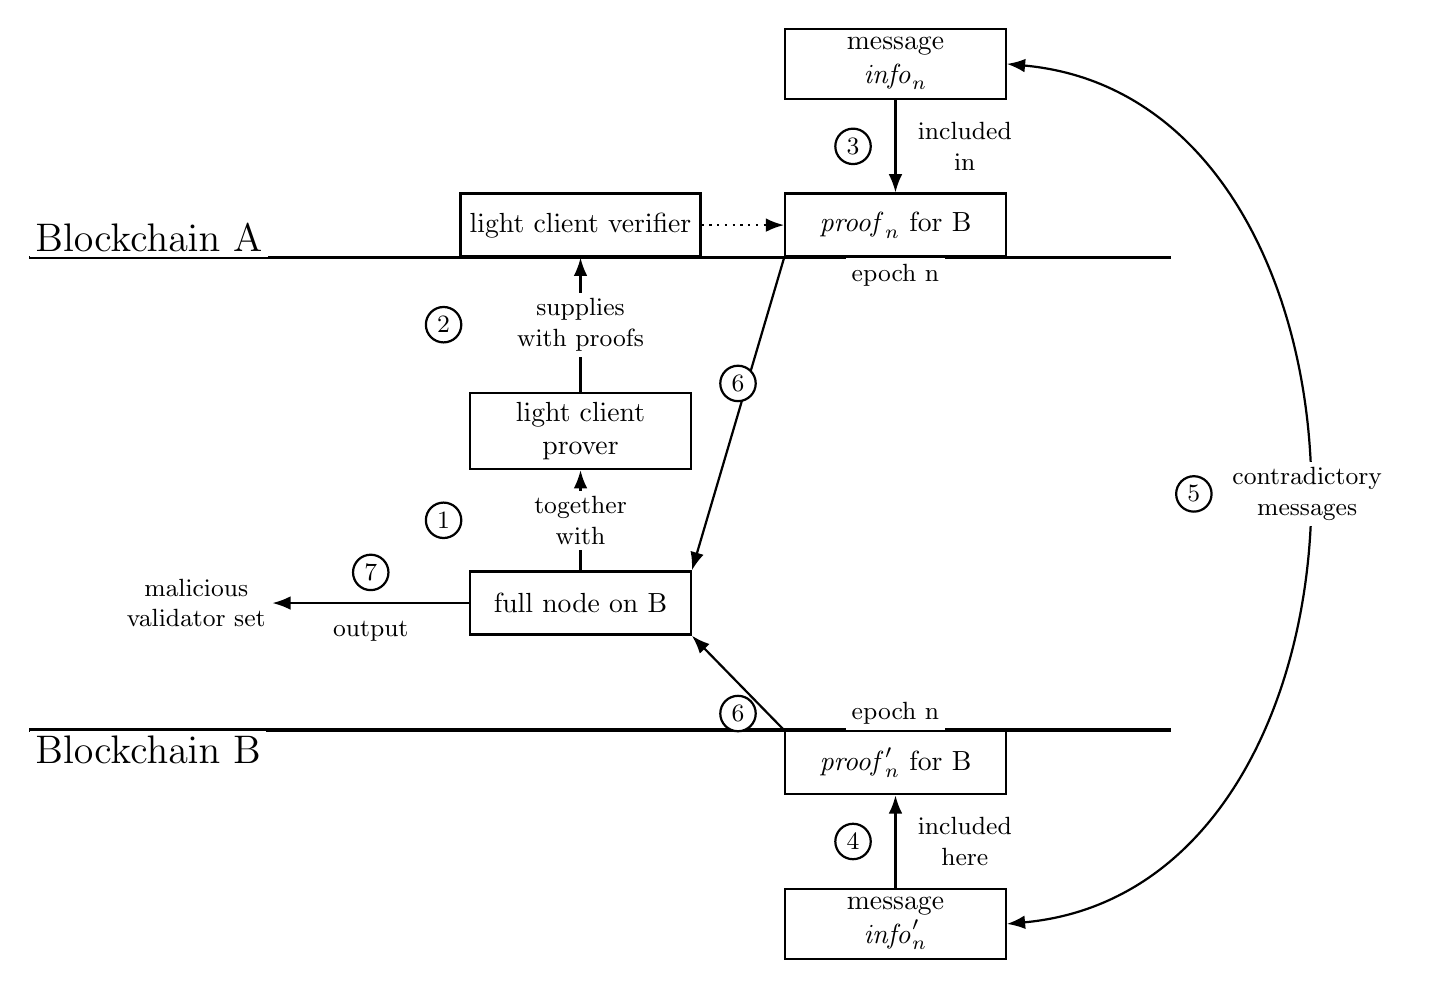
\begin{tikzpicture}[
    box/.style={draw, rectangle, minimum width=2.8cm, minimum height=0.8cm, align=center, thick, fill=white},
    circ/.style={draw, circle, inner sep=1pt, minimum size=0.45cm, font=\small, fill=white},
    txt/.style={align=center, font=\small, fill=white, inner sep=2pt},
    >=Latex % Arrow style
]

% -------------------------
% Blockchain A (Top Layer)
% -------------------------
% Boundary line for Blockchain A
\draw[very thick] (-1, 6.0) -- (13.5, 6.0);
\node[anchor=south west, font=\Large, fill=white, inner sep=2pt] at (-1, 6.0) {Blockchain A};

% Elements EXACTLY on line A (anchored 'south' at y=6.0)
\node (verifier) [box, anchor=south] at (6, 6.0) {light client verifier};
\node (proofA) [box, anchor=south] at (10, 6.0) {$\mathit{proof}_n$ for B};

% Dotted horizontal arrow between verifier and proofA
\draw[->, dotted, thick] (verifier.east) -- (proofA.west);

% "epoch n" exactly under the proofA box
\node (epochA) [txt, anchor=north] at (10, 6.0) {epoch n};

% Message info_n above
\node (msg1) [box, anchor=south] at (10, 8.0) {message \\ $\mathit{info}_n$};

% -------------------------
% Blockchain B (Bottom Layer)
% -------------------------
% Boundary line for Blockchain B
\draw[very thick] (-1, 0.0) -- (13.5, 0.0);
\node[anchor=north west, font=\Large, fill=white, inner sep=2pt] at (-1, 0.0) {Blockchain B};

% Box moved higher, clearly separated from line B (anchored 'south' at y=1.2)
\node (fullnode) [box, anchor=south] at (6, 1.2) {full node on B};
\node (proofB) [box, anchor=north] at (10, 0.0) {$\mathit{proof}'_n$ for B};

% "epoch n" exactly above the proofB box
\node (epochB) [txt, anchor=south] at (10, 0.0) {epoch n};

% Message info'_n below
\node (msg2) [box, anchor=north] at (10, -2.0) {message \\ $\mathit{info}'_n$};

% -------------------------
% Intermediary Layer: Prover
% -------------------------
% Moved higher, to y=3.8
\node (prover) [box, anchor=center] at (6, 3.8) {light client \\ prover};

% -------------------------
% Arrows and Connections
% -------------------------

% Arrow 1: From Full node to Prover
\draw[->, thick] (fullnode.north) -- (prover.south)
    node[midway, fill=white, txt] {together \\ with}
    node[midway, left=1.5cm, circ] {1};

% Arrow 2: From Prover to Verifier (Vertical, solid line)
\draw[->, thick] (prover.north) -- (verifier.south)
    node[midway, fill=white, txt] {supplies \\ with proofs}
    node[midway, left=1.5cm, circ] {2};

% Arrow 3: From info_n to proofA (Solid line)
\draw[->, thick] (msg1.south) -- (proofA.north)
    node[midway, right=0.2cm, txt] {included \\ in}
    node[midway, left=0.3cm, circ] {3};

% Arrow 4: From info'_n to proofB (Solid line)
\draw[->, thick] (msg2.north) -- (proofB.south)
    node[midway, right=0.2cm, txt] {included \\ here}
    node[midway, left=0.3cm, circ] {4};

% Arrow 5: Curve from info_n to info'_n (Contradictory messages)
\draw[<->, thick] (msg1.east) .. controls (16.5, 8.0) and (16.5, -2.0) .. (msg2.east)
    node[midway, fill=white, txt] {contradictory \\ messages}
    node[midway, left=1.2cm, circ] {5};

% -------------------------
% Slanted Arrows (Automatically directed to the new position of the full node on B)
% -------------------------
% From proof_n for B to full node on B (to the top-right corner of the box)
\draw[->, thick] (proofA.south west) -- (fullnode.north east)
    node[pos=0.5, above=0.15cm, circ] {6};

% From proof'_n for B to full node on B (to the bottom-right corner of the box)
\draw[->, thick] (proofB.north west) -- (fullnode.south east)
    node[pos=0.5, below=0.15cm, circ] {6};

% -------------------------
% Arrow 7: Malicious Validator Set Output
% -------------------------
% From the left of the full node box, horizontal arrow pointing left
\draw[->, thick] (fullnode.west) -- ++(-2.5, 0)
    node[midway, above=0.15cm, circ] {7}
    node[midway, below=0.15cm, txt] {output}
    node[left, txt] {malicious \\ validator set};

\end{tikzpicture}
\end{document}